\documentclass[12pt,oneside]{report}

%%% Load some useful packages:
%% "New" LaTeX2e graphics support.
\usepackage{graphicx}
%%	using final option to force graphics to be included even in draft mode
%\usepackage[final]{graphicx}
%% Tell graphicx the default directory for all figures
\graphicspath{{figures/}}

% Enable subfigure support
\usepackage{subfigure}

%% Make subsubsections numbered and included in ToC
\setcounter{secnumdepth}{3}
\setcounter{tocdepth}{2}

%% Package to linebreak URLs in a sane manner.
\usepackage{url}

%% Define a new 'smallurl' style for the package that will use a smaller font.
\makeatletter
\def\url@smallurlstyle{%
  \@ifundefined{selectfont}{\def\UrlFont{\sf}}{\def\UrlFont{\small\ttfamily}}}
\makeatother
%% Now actually use the newly defined style.
\urlstyle{smallurl}

%% Define 'tinyurl' style for even smaller URLs (such as in tables)
\makeatletter
\def\url@tinyurlstyle{%
  \@ifundefined{selectfont}{\def\UrlFont{\sf}}{\def\UrlFont{\scriptsize\ttfamily}}}
\makeatother

%% Provides additional functionality for tabular environments
\usepackage{array}

%% Puts space after macros, unless followed by punctuation
\usepackage{xspace}

%% Make margins less ridiculous
\usepackage{fullpage}

%% Allows insertion of fixme notes for future work
\usepackage[footnote, nomargin]{fixme}

%%%% Turned off for tech report, should be turned on for research portfolio
%% Turn on double spacing
\usepackage{setspace}
\usepackage{mdwlist}
\doublespacing

%% Make URLs clickable
%\usepackage[colorlinks, bookmarks=false]{hyperref}
\usepackage[colorlinks, bookmarks=true]{hyperref}

%% Since I'm using the LaTeX Makefile that uses dvips, I need this
%% package to make URLs break nicely
\usepackage{breakurl}

\usepackage{todonotes}
\usepackage{amsmath,amsfonts}
\numberwithin{equation}{subsection}
%%\usepackage{nonfloat}
\usepackage{bbm}
\usepackage{setspace}
\onehalfspacing
\usepackage{tabularx}

%%% End of preamble
\begin{document}

\begin{titlepage}
\vspace*{1in}
\begin{center}
   
\Large


{\bf Project Hackystat: Accelerating adoption of empirically guided software development through
  non-disruptive, developer-centric, in-process data collection and analysis}

\bigskip

\normalsize

Philip Johnson                           \medskip\par
Department of Information and Computer Sciences\\ 
University of Hawaii\\ 
Honolulu, HI 96822\\                       
(808) 956-3489\\
(808) 956-3548 (fax)\\
{\tt johnson@hawaii.edu}                 \bigskip\par

\today                                   \bigskip\par



\end{center}
\end{titlepage}


%% Philip suggests it needs a ToC
\tableofcontents

\begin{abstract}
%Abstract goes here if needed.
Software process defines a structure imposed on a human activity resulting in a software. 
Many different kinds of software processes were designed up today, however they are not
proven to deliver consistently and fail with equal probability. 
This phenomena was widely observed and identified as a ``software crisis'' in 1968 and 
since then it was the subject of numerous research aiming the process control and improvement. 
Today formal pocess models, standards, guidlines and recomendations provide teams 
and individuals with easy-to-understand methodologies and allow a great flexibility of 
processes for project needs, but the rate of failing software projects remains about the same. 
Recently, as an alternative opinion - the ``software development process as a craft'' 
idea emerged - this approach emphasizes roles of highly motivated, creative and skilled
individuals in software creation. Software craftsmanship paradighm of software processes 
finding  some strong supporters in the industrial and research communities recently. 

However both views, while supported by excellent research work and industrial success stories, 
follow conventional ``top-down'' technique - at first someone has to invent a
process, design and implement its building blocks and empirically evaluate it after. 
The problem with this approach, as shown in \cite{citeulike:9758924} by van der Alast,
is that one assumes an idealized versions of real processes and tend to produce 
``paper lions'' - process models which are likely to be disruptive and unacceptable for end users.

In my work I explore an alternative approach for the software process analysis - 
through the discovery of recurrent behaviors (habits) from software process artifacts trails.
Previously it was shown that it is possible to automatically recognize \cite{citeulike:2703162} 
test-driven development patterns, in my work I expand this previous experience by intoducing and 
exploring the applicability of a new temporal data mining technique in oder to find 
unknown recurrent behaviors in the space of all possible permutations of existing processes. 
Finding and understanding these recurrent behaviors may shed light on programming 
habits and their role and interactions within a software process.
\end{abstract}

% my main text chapters
\chapter{Introduction}
Delivering high quality software products within the budget and in time is the main goal and the most 
challenging task of Software Engineering. Years of scientific research in this area resulted in a 
number of software processes providing detailed guidelines on how to reach 
the goal efficiently. These processes manifested themselfs as the means for improvements in terms 
of quality, speed and cost over existing practices. Many were implemented and tested within academic 
and industrial settings and proved proposed superiority. Some of these processes were successfully 
adopted and standardized in industry shaping the best practices of contemporary software development 
\cite{citeulike:9962021}. Moreover, there are plethora of processes for improving existing processes 
of software development on the team \cite{citeulike:9962027} and personal 
levels \cite{citeulike:9962022}.

The processes I am mentioning here are the well-known large formal models such as Waterfall and Spiral, 
as well as more flexible iterative agile approaches like XP, SCRUM or FDD. These are also sets of 
rules and recommendations which can be applied to certain stages of the software processes 
such as Test Driven Development or Pair Programming; there are general guidelines helping 
to improve the correctness of a product and standards, like CMMI or ISO 9000; guidlines for testing 
and measurements, code syntax rules and formatting styles, code comments 
recomendations \cite{citeulike:900855}. 

From the first sight, taking all this in account,  one would guess that 
the area of software processes is thoroughly explored and there are clear choices of processes 
and models for the one in charge making decision... But it is not true - despite many choices 
one can make, no one can foretell what is the ``best'' process to choose for certain constraints.
What managers are left with are the equal alternatives and vague promises. 
This deficiency in knowledge is the main coause of the ``software crisis'' phenomena point is supported by the fact that according to ``Chaos Report'' from the Standish 
Group (Rubinstein) \cite{SDTimes} only ``35\% of software projects in 2006 can be categorized as successful - meaning 
they were completed on time, on budget and met user requirements''. 
These thirty five percent of success clearly saying that it is somewhat difficult to make 
a statement that we are fully understand and able to control software processes. 
Moreover, over years, while this idea of a software process formalizations shaped the 
programming practices, which once thought to be a creative human activity accessible by amateurs 
and hobbyists \cite{citeulike:9958822} into a serious engineering discipline, bounded 
by requirements for education, standardized processes, rules, certifications, and strict 
financial requirements from stakeholders the opposite idea was born - the idea of 
software development as a craft. Interesting that such a duality of views can be found 
in the work of a single person \cite{citeulike:5203446}.

Clearly, there is a great room for research and improvement of our understanding of software processes.
This exploratory study is yet another attempt at the understanding. In my research work I am 
exploring techniques aiming the understanding of small processes which are 
rather the reflection of personal behaviors or habits of software development rather than a 
formalized constructs. Also, I would like to emphasize, that in this work I will not 
address the need and means of the process synthesis, its quality assessment, productiveness
or any topics related to the software product itself; I would rather focus on the specific issue - 
uncovering an existence and studying the programming habits. 

This thesis presents a methodology for finding recurrent behaviors through the 
analysis of the variety of software process artifacts left after performing a 
software process. I have called this methodology ``Software Trajectory'' and it consists 
of four distinct steps. Each of these steps has a specific goal and compromising variety of 
means to reach it. 
At first software process artifacts are identified and collected. 
At second, they are cleaned, organized and classified. 
On the third step particular research questions are formulated and data are organized and indexed. 
And finally, a set of KDD techniques is applied in order to undercover recurrent behaviors which 
could potentially shed a light on the performed process details. 

My personal motivation for performing this work is coming from the recognition of the 
importance of the software in our lives and the severity of issues with its development. 
Through my everyday experiences with software development and use I have stumble upon 
a number of issues which made me realize that mentioned ``software crisis'' phenomena is very real.
As a user in industrial and academic settings I often find myself facing software failures 
which create numerous difficulties for reaching production or research goals. As a developer, 
in an attempt to be productive and in order to deliver a better software I have studied and 
explored a number of formal processes, however, sometime I found myself seeing a very little of 
rationale behind their application, and moreover, in this exploration, when facing the process
application failing to help I was unable to comprehend what exactly went wrong and what need 
to be changed. All of these experiences made me studying software process research and exploring
novel approaches to software process recovery on my own in order to understand software process better.

\section{Research area overview}
As mentioned above, in this thesis I am focusing on a very narrow subject - exploring approaches
for uncovering of recurrent behaviors or ``programming habits'' out of software process artifacts.
Before narrowing further 


Software is usually coded by teams. Members of these teams are agreed and bound to use 
a particular technologies and development tools, they also agree on following well defined 
development process which is constrained by a timeline and budget. These are necessary 
constraints to keep work organized, however there is a great freedom in what they actually 
do in every single moment of time in order to progress towards lines of code which eventually 
will result in software. For example one developer may follow test first process while
another writes tests at last.  This freedom of choice in ordering of development activities 
while being much appreciated by talented and creative individuals creates an impression 
of chaotic and unordered activities for random observers, newbies and people in 
charge - so there we have all the attempts of imposing an order 
(or control) on all of the development activities. Metrics and models of processes





\chapter{Software Process}
There are different approaches for software development which were designed in order to 
facilitate the creation of software systems. Regardless of the chosen approach the 
process of software creation includes three generic phases: definition phase, 
development phase and a maintenance phase \cite{citeulike:6095377}.
The definition phase includes the initial
planning of the future system and requirements collection. Developers identify data 
need to be processed by the system, its functionality, behavior, and what are 
the constraints there are in the design and development. The development phase focuses 
on the system implementation and its testing. Developers write the system code, 
test if the system satisfies planned requirements in the behavior and and output. 
The maintenance phase focuses on the post-development activities: system deployment 
and its operational support. 

Another common part of these approaches is the use 
of a software process model and following a software method, also known as methodology.
While latter is used to primarily navigate through the development process determining
a number of functional points, designing data flow diagrams etc., the model provides 
developers with guidance about their tasks and the activities that should be undertaken 
during development. It is advocated that the use of established and well structured 
model is crucial for the complex projects in order to orchestrate collaborative effort 
of multiple teams. 

These models can be characterized by the series of distinct phases, in fact, the 
determination of phases, its ordering and the definition of the phase-transitioning 
criteria are the core model components.
Each of these phases is executed with a particular goal: some will provide a part of the 
software system, other will deliver engineering documentation or a user manual, or 
validate an existing code. Examples of such phases are the requirements collection, 
user manual writing or the coding of a functional module of the software system. 
While the methodology prescribes an ordering of carried activities, it also facilitates
a framework for estimation of needed resources, defines major milestones, and provides 
means for time and effort monitoring and management. 

In this chapter I will review major of existing software process models providing additional 
information about their derivatives and discussing their strengths and weaknesses.
The purpose of this narrowing is to present the current state of the art in software 
processes.

\section{Code-and-fix model}
According to Boehm \cite{citeulike:10002126}, the pioneering days of software development 
industry can be characterized by the application of the code-and-fix methodology
which covered full software life cycle. This model essentially consisted of two phases:
write some code and fix problems in the code. Professional programmers as well as enthusiasts 
were coding implementations of their ideas first and spent time iteratively adjusting the 
code to the requirements or errors fixing later. While being intuitively transparent, this 
approach led to the number of problems - after a number of fixes, enhancements and 
work-arounds code become unreadable and very expensive to maintain; also non-existence of
distinct testing phase allowed bugs to persist until they were revealed by the end-users.

\begin{figure}[tbp]
   \centering
   \includegraphics[height=60mm]{model_00_code_and_fix}
   \caption{The code-and-fix model \cite{citeulike:10002126}.}
   \label{fig:code_fix_model}
\end{figure}

\section{Stagewise model}
Through the experience with code-and-fix approach the need for requirements collection and 
for design phase prior to coding become evident as well as the need of structured 
testing and evaluation. The recognition these needs by the industry and the first experiences
with development of large software systems such as Semi Automated Ground 
Environment \cite{citeulike:10004001} \cite{citeulike:10004037} led to the development 
of stagewise software model by Benington (1956) \cite{citeulike:10004032}. 
This model consisted of a number of stages:
\begin{itemize}
 \item Operational plan
 \item Operational specifications
 \item Coding specifications
 \item Coding
 \item Parameter testing
 \item Assembly testing
 \item Shakedown
 \item System evaluation
\end{itemize}
These stages were streamlined as a sequential process - every completed stage created a
grounds for its successor. While seem to be naive, this formalization of the process was a 
significant breakthrough at the time. Soon it was recognized, that this unidirectional process
doesn't stipulate what to do if the rework of previous stage(s) is necessary - there was 
no formalization of such iterations and the revision of the model was requested.

\section{Waterfall model}
The Waterfall model is probably the oldest and the most influential of existing software 
process models and it is very popular in the domain of development of large and 
complex software systems. 
This model is a refinement of a stagewise model and its 
original version is credited to Royce (1970) \cite{citeulike:9982731}. There were two 
changes from the predecessor - first was a recognition of the feedback loops between 
stages and its limitation to successive stages only - in order to exclude expensive
cross-stage rework, while the second change was the inclusion of a prototyping stage
\cite{Boehm95anchoringthe}.

\begin{figure}[tbp]
   \centering
   \includegraphics[height=87mm]{model_01_waterfall}
   \caption{The waterfall software development model. Solid lines represent a staged 
      model implementation with no feedback. Dotted lines add a possibilty of 
      iterative transition between adjacent stages. Dashed line show model 
      implementation with feedback \cite{citeulike:9982731}. }
   \label{fig:model_waterfall}
\end{figure}

Waterfall model is an example of a plan-driven process - one must plan and schedule all 
of the activities before their execution. Model has many variations and the approach 
articulated by the model forms the basis of many standards in the software industry.

There is successive and distinct progression of stages in waterfall model; each state 
is well defined and forms the basis for the successive one. In addition to specific 
deliverable, each state producing a document which describes what exactly occurred 
during the stage, providing certain visibility to the processes, and facilitating 
audit. Each state has milestones and deliverables explicitly defined.

Five stages of waterfall model reflect the fundamental development activities:
\begin{enumerate}
 \item \textit{Requirements analysis and definition.} The feasibility study 
is conducted 
and the requirements collected. The system functionality clarified and
documented in details - the requirements specification document - delivered  
and will serve as the system specification. It is assumed that customer's 
expectations are articulated and will not change much throughout the development 
process.
 \item \textit{The system design.} Within this phase requirements for hardware and 
software components defined by the establishing an overall system architecture.
All system modules and their interactions are designed in accordance with 
collected requirements.
 \item \textit{Implementation and unit testing.} The actual code produced, individual 
modules are tested individually. This phase embeds all quality control checks.
 \item \textit{Integration and system testing.} System assembled and once complete, it
is tested and evaluated in actual conditions (alpha tested).
 \item \textit{Delivery and Maintenance.} System is tested by actual customer(s) 
(beta testing). Identified errors are corrected and if found satisfiable, 
software system is installed and put into use. Maintenance involves error correction, 
improvements of system units and enhancements of services if desired.
\end{enumerate}

During transition from stage to stage within the waterfall model, previous state 
should be signed-off - approved to be in finished state. In other 
word, states should not overlap, however in the real life problems often discovered
later on - for example it is often happens that problems with design 
discovered only after implementation is started and so on. In such situation
process returns to the problematic phase and changes are made and reflected in 
the documentation. These iterations are very costly in time and effort and 
usually after a certain number of iterations problematic stages considered 
``frozen'' and development continues. Identified and not resolved issues persist
through the further work and if possible - covered by workarounds, if not - 
they just ignored and system may not perform correctly or lack some functionality 
afterwards.

The big advantage of waterfall model of software development process is that 
it is consistent with other engineering models in terms of general approach, 
its flow and produced documentation. It seems to be manager-friendly too since
it is easy to track the progress against the development plan. The major 
problem with this model is
that within such a specification-based approach stakeholders finding it 
extremely difficult to articulate their requirements in advance and 
that requirements changes are very hard to incorporate after first stages are passed.

In 1988 Boehm revisits waterfall model and after re-stating its fundamental problems 
offers three classes of improved software process models - evolutionary development 
model, the transform model and the spiral model \cite{citeulike:10002126}.

\subsection{Evolutionary development model}
Evolutionary development proposed by McCracken\&Jackson in 1982 \cite{citeulike:3996892}
was among the first reactions to the waterfall model's problems. Instead of moving 
through well-defined stages and producing number of documents, it claims the only
stage - release of extended system capability which is a response to the user 
requirements and is based on the operational experience. Evolutionary paradigm 
is built around early release of the pre-operational product (prototype) and its gradual 
enhancement (evolutional development) through feedback. 

Within the evolutionary development model stakeholders are provided with a somewhat 
functioning software system at the very beginning and their feedback directs all future
software system enhancements. This model perfectly matches the user expectations 
about the software requirements evolution - gradually, through everyday experiences, 
as an opposite to waterfall model upfront requirements collection. 

However, this is what fails in evolutionary development - the new model was found 
stigmatized with weaknesses of the old code-and-fix approach - spaghetti code and 
the lack of formal planning - the exact reasons waterfall model was invented... 
And in addition evolutionary development does not provide any means for identifying 
and fixing early erroneous design decision - instead it encourages working around 
major issues which inevitably creates large expensive to maintain codebase instead 
of re-considering early decisions.


\subsection{Spiral model}
The spiral model reflects the concept in which each of development cycles involves a 
progression addressing the same sequence of steps as in previous level. The figure 
\ref{fig:model_spiral} illustrates the model representation as a spiral according 
to Boehm \cite{citeulike:10002126}. Each loop of this spiral represents a phase of 
software process. Innermost loop concerns the system feasibility study. The second 
loop represents a system requirements definition and system design and so on. 
The radial (Y) dimension represents a cumulative cost of the system up to date, 
while angular dimension represents a loop progress towards completing the current 
spiral loop.

\begin{figure}[tbp]
   \centering
   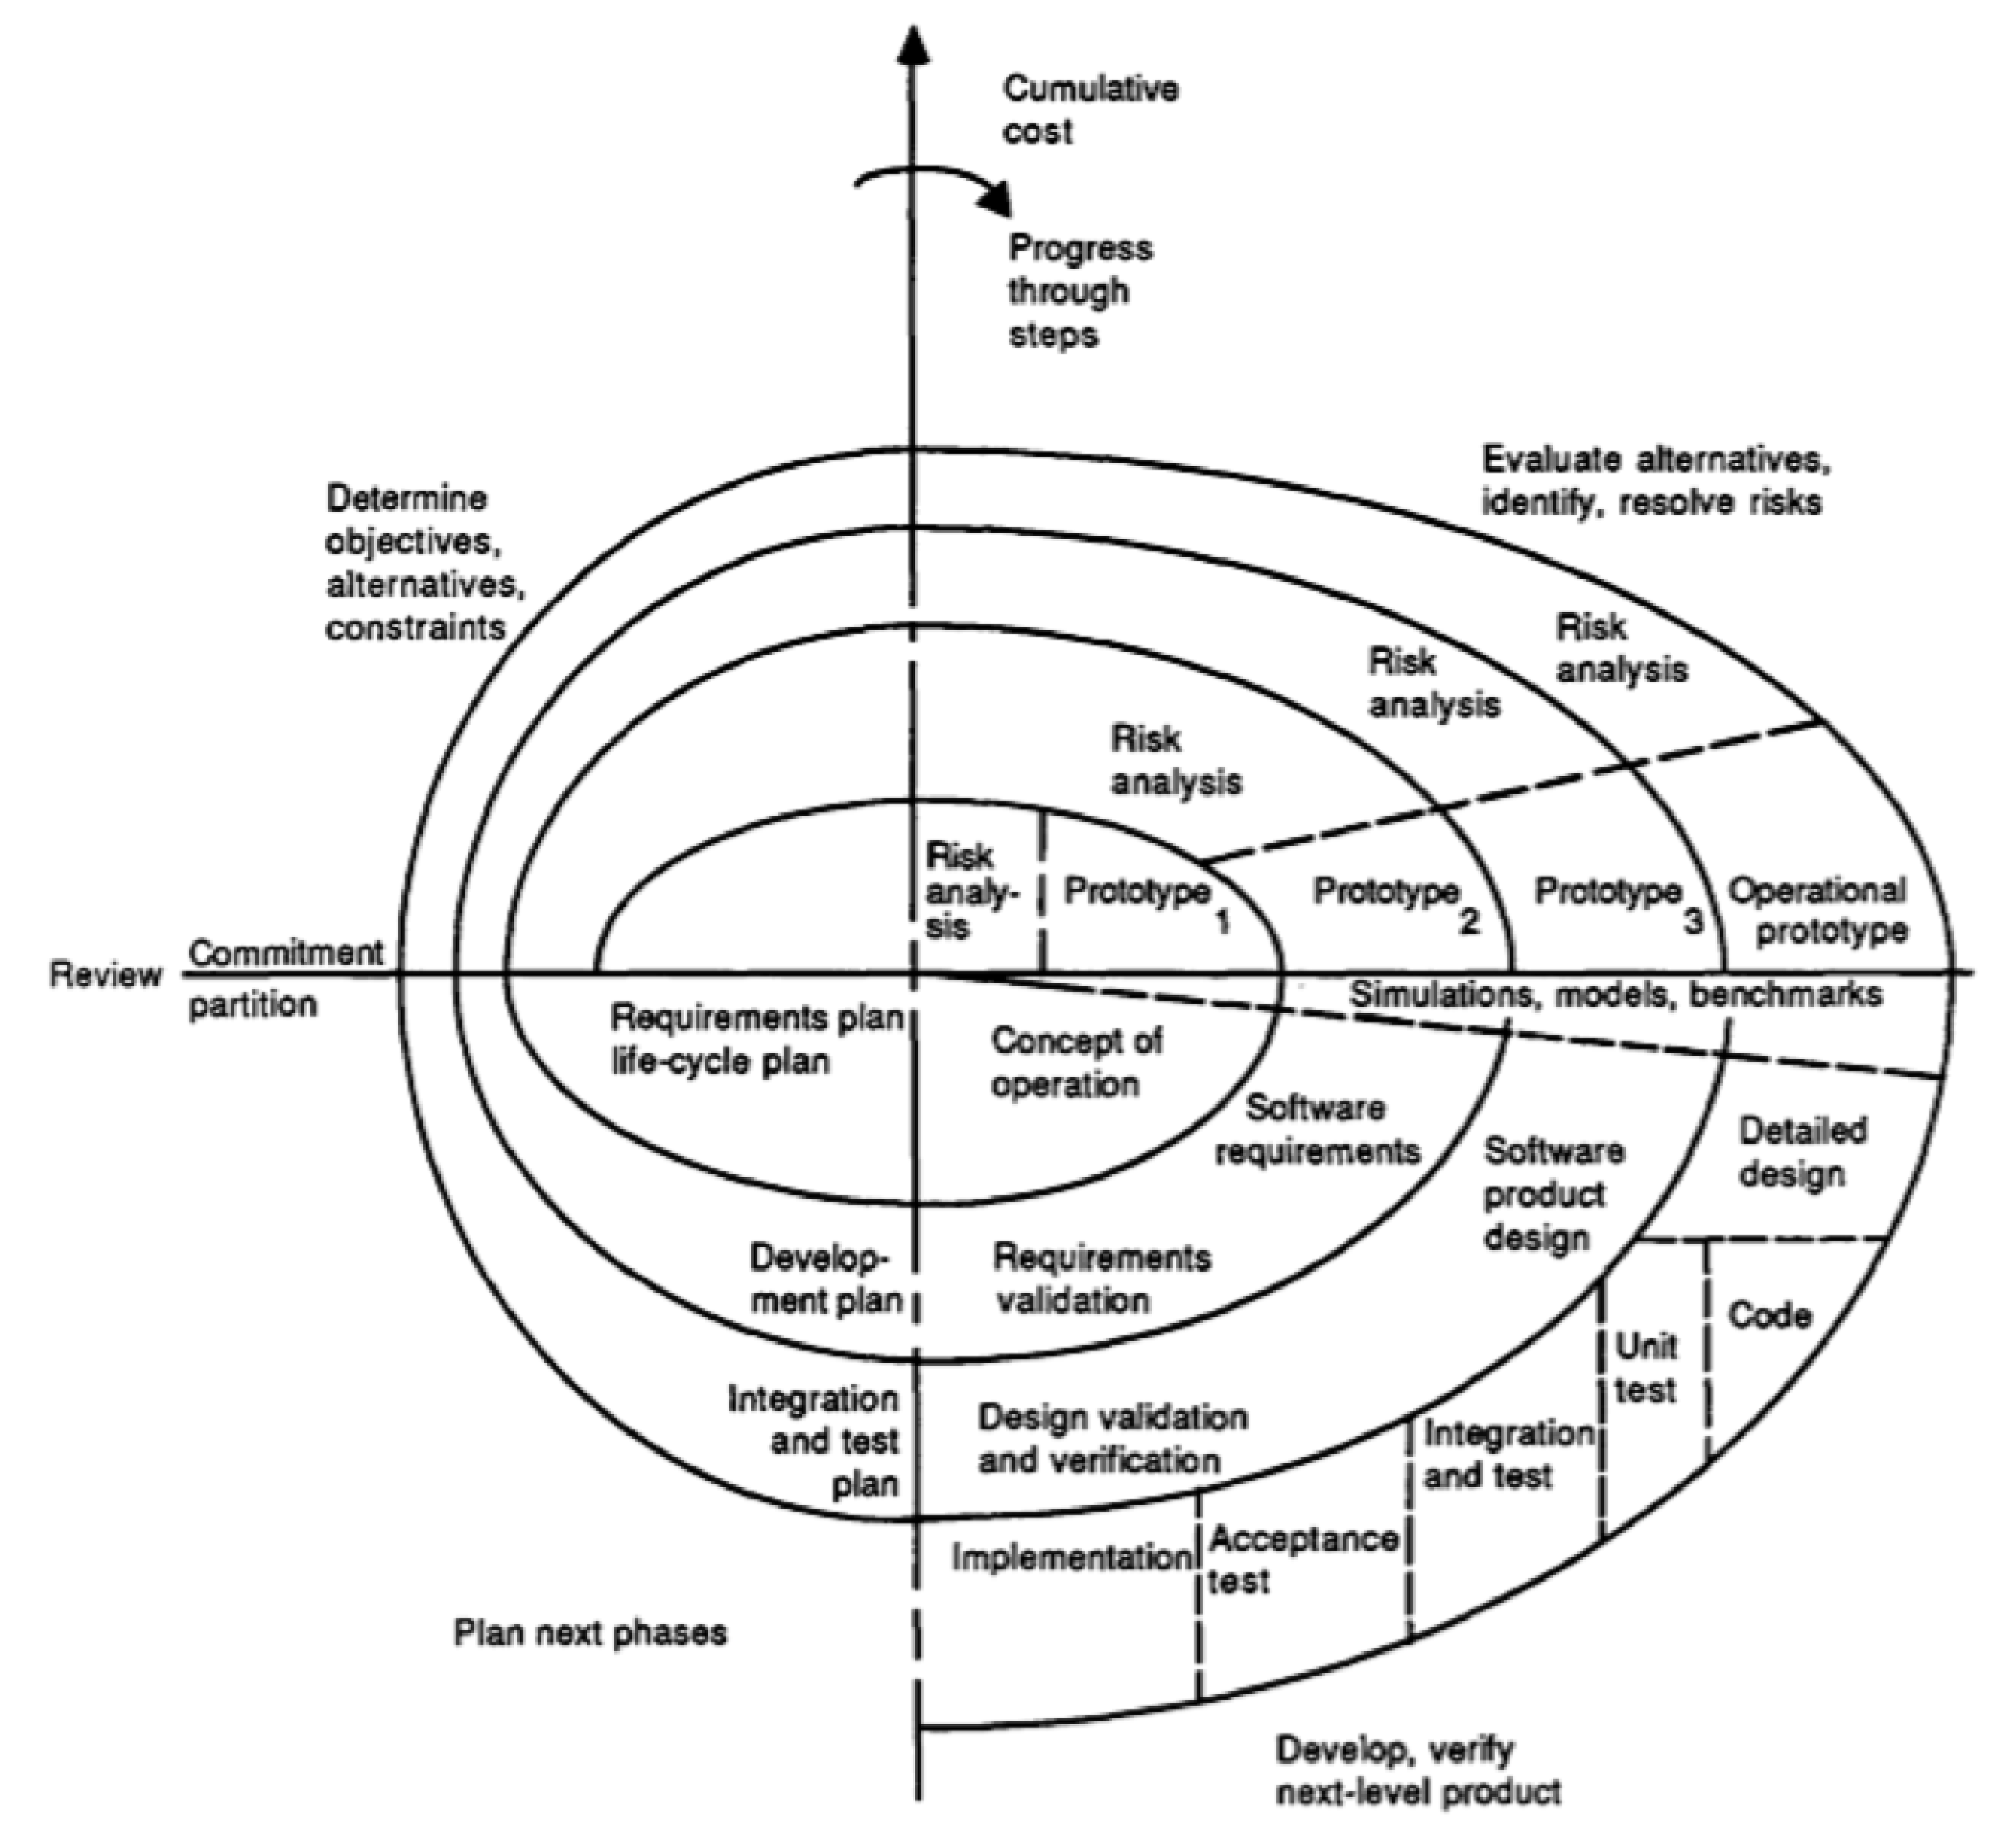
\includegraphics[height=150mm]{model_02_spiral-boehm}
   \caption{The spiral model of software development according to Boehm \cite{citeulike:10002126}. }
   \label{fig:model_spiral}
\end{figure}



\subsection{Cleanroom software engineering}
Another of waterfall model derivatives is a Cleanroom development methodology, which is
a fusion of waterfall model with formal methods approach. 
Following the formal methodology, stages of waterfall model reshaped into 
\begin{enumerate}
 \item \textit{Formal specification} phase, where the software system is presented as 
a state-transition model with input and output. The states of the system and
its transitions (reactions on input) reflect specification and requirements.
 \item \textit{Structured, incremental development} phase. By application of the 
cleanroom methodology the software is partitioned into increments using the 
specification and the development process Within cleanroom
development process only a limited amount of programming constructs allowed,
and the development process is an iterative refinement of specification
\end{enumerate}

1) formal specification phase; 2) incremental, formal development and verification 
, formal methods are a particular kind of mathematically-based techniques for
the specification, development and verification of software and hardware systems

\section{}

It is currently well recognized in the software industry that the process of software development 
is critical to the success of any major development project.
The Institute of Electrical and Electronics Engineers defines software engineering as 
“the application of a systematic, disciplined, quantifiable approach to development, 
operation, and maintenance of software; that is, the application of engineering software”

\chapter{Process Mining}

\section{Software Process Recovery}
Software development process was always being under focus of various stakeholders due to the number of reasons ranging from standards compliance to business and security intelligence. When no live observations are made on the performers, due to the availability, timing, cost, or privacy issues, recovering software process from artifacts could be complex and expensive process. Researchers have suggested a possibility of software process recovery by interviewing of developers and managers and by analysis of process artifacts: such as printed documents - designs, use-cases, software inspections or electronic artifact trails: version, bug and issue control systems and mailing lists. This research resulted in many published work:
\begin{itemize}
\item{Cook \& Wolf in \cite{citeulike:328044} discuss an event-based framework for process discovery based on grammar inference and finite state machines. The authors directly applied their framework to Software Configuration Management (SCM) logs demonstrating satisfactory results.}
\item{Jensen \& Scacchi \cite{citeulike:5043664} describe an interesting framework built upon mapping between process artifacts and process entities into an universal generic meta-model. Application of their human-involved technique leveraged a pre-existing domain knowledge for the effective pruning and iterative process revision resulted in ``workflows discovery''.}
\item{German in \cite{citeulike:421438} performed a manual mining of the GNOME process artifacts: documentations, CVS logs, and one hundred and four mailing-lists in order to
describe the development processes from GSD (Global Software Development) point of view.}
\item{Ripoche tried a more automatic approach in \cite{citeulike:9112798} by developing a generic model for process-based explanation of bugs persistence using state diagrams and
probabilistic choices.}
\end{itemize}
All these suggests that software process artifacts bear enough information about performed process for its recontsruction. In my study I havily relying on this fact. This not only serves as a foundation of my hypothesis, but also partially assures the validity of my approach to the software process reconstruction. Further in this chapter I will introduce a novel technique of pattern mining form the software process artifacts trails. After introduction of the technique, I will walk through the performed case studies in which I have applied this technique to the various types of the software process artifact trails.

\input{method_apriori}

\section{Symbolic Aggregate approXimation (SAX)} \label{sax}
\begin{figure}[tbp]
   \centering
   \includegraphics[height=45mm]{sax_intro}
   \caption{The illustration of the SAX approach taken from \cite{citeulike:2821475} depicts two pre-determined breakpoints for the three-symbols alphabet and the conversion of the time-series of length $n=128$ into PAA representation followed by mapping of the PAA coefficients into SAX symbols with $w=8$ and $a=3$ resulting in the string \textbf{baabccbc}.}
   \label{fig:sax_intro}
\end{figure}

Symbolic Aggregate approXimation was proposed by Lin et al. in \cite{citeulike:2821475}. This method extends the PAA-based approach \cite{citeulike:2946589} \cite{citeulike:3000416}, inheriting algorithmic simplicity and low computational complexity, while providing satisfiable sensitivity and selectivity in range-query processing. Moreover, the use of a symbolic representation opens the door to the existing wealth of data-structures and string-manipulation algorithms in computer science such as hashing, regular expression pattern matching, suffix trees etc.

SAX transforms a time-series $X$ of length $n$ into a string of arbitrary length $\omega$, where $\omega << n$ typically, using an alphabet $A$ of size $ a \geq 2$. The SAX algorithm consist of two steps: during the first step it transforms the original time-series into a PAA representation and this intermediate representation gets converted into a string during the second step. Use of PAA at the first step brings the advantage of a simple and efficient dimensionality reduction while providing the important lower bounding property as shown in the previous section. The second step, actual conversion of PAA coefficients into letters, is also computationally efficient and the contractive property of symbolic distance was proven by Lin et al. in \cite{citeulike:532335}.

\begin{equation}
D_{PAA}(\bar{X}, \bar{Y}) \equiv \sqrt{\frac{n}{M}} \sqrt{ \sum_{i=1}^{M} 
\left(  \bar{x}_{i} - \bar{y}_{i} \right)}
\label{eq:paa_distance}
\end{equation}

Discretization of the PAA representation of a time-series into SAX is implemented in a way which produces symbols corresponding to the time-series features with equal probability. The extensive and rigorous analysis of various time-series datasets available to the authors has shown that normalized by the zero mean and unit of energy time-series follow the Normal distribution law. By using Gaussian distribution properties, it's easy to pick $a$ equal-sized areas under the Normal curve using  lookup tables  \cite{citeulike:4434481} for the cut lines coordinates, slicing the under-the-Gaussian-curve area. 
The $x$ coordinates of these lines called ``breakpoints'' in the SAX algorithm context. The list of breakpoints $B=\beta_{1}, \beta_{2}, ... , \beta_{a-1}$ such that $\beta_{i-1} < \beta_{i}$ and $\beta_{0} = -\infty$, $\beta_{a} = \infty$ divides the area under $N(0,1)$ into $a$ equal areas. By assigning a corresponding alphabet symbol $alpha_{j}$ to each interval $[\beta_{j-1},\beta_{j})$, the conversion of the vector of PAA coefficients $\bar{C}$ into the string $\hat{C}$ implemented as follows:
\begin{equation}
\hat{c}_{i} = alpha_{j}, \; \text{iif} \; \bar{c}_{i} \in [\beta_{j-1},\beta_{j})
\label{eq:alpha}
\end{equation}

\begin{figure}[tbp]
   \centering
   \includegraphics[height=47mm]{sax_distance}
   \caption{The visual representation of the two time-series $Q$ and $C$ and three distances between their representation: Euclidean distance between raw time-series (A), the distance defined for PAA coefficients (B) and the distance between two SAX representations (C). (The figure taken from \cite{citeulike:2821475} as well)}
   \label{fig:sax_distance}
\end{figure}

SAX introduces new metrics for measuring distance between strings by extending Euclidean and PAA (\ref{eq:paa_distance}) distances. The function returning the minimal distance between two string representations of original time series $\hat{Q}$ and $\hat{C}$ is defined as
\begin{equation}
MINDIST(\hat{Q},\hat{C}) \equiv \sqrt{ \frac{n}{w} } \sqrt{ \sum_{i=1}^{w} ( dist( \hat{q}_{i}, \hat{c}_{i} ) )^{2}}
\label{eq:sax_mindist}
\end{equation} 
where the $dist$ function is implemented by using the lookup table for the particular set of the breakpoints (alphabet size) as shown in Table \ref{tbl:sax_lookup}, and where the singular value for each cell $(r,c)$ is computed as 
\begin{equation}
cell_{(r,c)} = 
\begin{cases} 
0, \text{ if }\left| r-c \right| \leq 1 \\
\beta_{\max(r,c) - 1} - \beta_{\min(r,c) - 1}, \text{ otherwise}
\end{cases}
\label{eq:cell}
\end{equation}

\begin{table}
\begin{tabularx}{400pt}{X X X X X}
\hline
   & a   & b    & c    & d    \\
\hline
a & 0    & 0    & 0.67 & 1.34 \\
b & 0    & 0    & 0    & 0.67 \\
c & 0.67 & 0    & 0    & 0    \\
d & 1.34 & 0.67 & 0    & 0    \\
\hline
\end{tabularx}
\caption{A lookup table used by the MINDIST function for the $a=4$}
\label{tbl:sax_lookup}
\end{table}

As shown by Li et al., this SAX distance metrics lower-bounds the PAA distance, i.e.
\begin{equation}
\sum_{i=1}^{n} (q_{i} - c_{i})^{2} \geq n(\bar{Q} - \bar{C})^{2} \geq n(dist(\hat{Q},\hat{C}))^2
\label{eq:sax_bounding}
\end{equation}

The SAX lower bound was examined by Ding et al. \cite{citeulike:4501572} in great detail and found to be superior in precision to the spectral decomposition methods on bursty (non-periodic) data sets.



\chapter{Software artifacts}
Software development activity leaves many artifacts. The variety depends on the complexity of the project 
as well as on the software process model followed by developers. Typical formal artifacts include the 
following: 
\begin{itemize}
 \item Sytem specification documents
 \item Software project plan
 \item Software requirements specification
 \item Software design specification
  \begin{itemize}
   \item Data flow design specification
   \item Interface design specification
   \item System architechture specification
  \end{itemize}
 \item Source code
 \item Code review reports
 \item Software test specification
  \begin{itemize}
   \item Test plan
   \item Test cases and test data
   \item Test reports
  \end{itemize}
 \item Installation manual (administration manual)
 \item User manual
 \item Maintenance documents
  \begin{itemize}
   \item Bug reports, feature requests
   \item Change reports
  \end{itemize}
\end{itemize}
Along with formal set of artifacts, there is a variety of informal artifacts. These include SCM system logs
developers mailing list archives, exchange not designed 
and produced to be formally or automatically analyzed

\section{Software configuration management}
Software evolve. The software evolution happens under the pressure from stakeholders, end users and due to the infomation technology evolution. It is practically inevitable.
\todo[size=\tiny]{Here I need to narrow the need of SCM and the evolution of software}
``Software configuration management'' or SCM (also known as ``software change and configuration management'') is a term used to descibe means of software evolution control by
software developers. These include but no limited to standards, approaches, techniques and tools for initiating, evaluating, and controlling change of software product before,
during and after the development process. Configuration management is an integral part of the software process spanning across all its phases and providing stucture and control
imposed on the software change, thus enabling it to be performed in a way which is reproducible and does not destroy the integrity of software.

Recalling the discussion of Goals of SCM will clearly paint a picture of what basic features an ideal SCM Tool should have in it.
•       First and most basic functionality a Software Configuration Management tool should provide is support for a central file repository. All other functionalities are around
managing and tracking of these repository items.
•       Secondly it is important that the SCM tool provides the capabilities of the distributed team to work together from a central repository. Features like file locking
mechanism, file comparison and atomic commits are to name a few.
•       The SCM tool should also provide a simple mechanism for creating and maintaining private branches and for merging changes from the main code line to the private branch, and
vice versa.
•       The SCM tool should provide visibility into changes made for each task and support the ability to work by task instead of by individual file, to merge changes from one
configuration to another, and to revert changes for a task if needed.
•       The SCM tool should also provide an easy mechanism for rolling back to the last good integration version.
•       The SCM tool supports simple creation of a hierarchy, give visibility into the changes at each stage, and enable straightforward merging between stages.
•       Tagging is another feature very common and useful which involves giving meaningful names to specific revisions. These names are generally called Tags or Labels.
•       The SCM tool should support re-targeting features without the need to write and maintain scripts to perform the operations.
•       In order to re-factor code and still be able to trace through the history of changes, an SCM tool must support file and directory rename and move operations and track the
operations as part of the element’s history.
•       The SCM tool should easily integrate with the continuous integration server so that latest code from the SCM repository can be extracted and compiled continuously and whole
process can be automated.


\chapter{Software Process Discovery}
\section{Software process recovery from SCM system}
As Ball et al. \cite{citeulike:9004378} and Zimmermann \& WeiBgerber \cite{citeulike:5058462} point out - all of the contemporary version control systems provide considerably large amount of auxiliary information about software change. In particular, version control system, when coupled with a mailing lists and (or) bug and issue tracking system is capable of providing information \textit{who} changed \textit{what} and \textit{why}. Which seems to be a fair amount of information needed for one's opinion about the change. It is possible to get an overall understanding of the change necessity through the analysis of bug and issue reports. Version control itself provides quantitative data about files and LOC and changed, added or deleted. The analysis of code snapshots (versions) allows to quantify the change in terms of various software metrics like complexity, cohesion etc. When considered in time all this data provides a solid background for a software evolution research.

However, what is very difficult to know from any contemporary SCM system is that a software process behind the changes. Nevertheless many research in the field of MSR was done in order to shed a light on the software process itself. \cite{citeulike:9007622} There are only traces of such information present in version control transactions. In order to recover some insights about the performed software process information behind a software change statistics behind the change can show us some behavioral patterns blanks in the single transactions can be restored by statistics
outliers effect can be diminished by statistics


\chapter{Case Studies}

\input{case_eclipse}

\chapter{Conclusions}
The ultimate premise of STA is to provide means for empirical guidance of developers and project 
management in software process execution and decision-making improvement.


%%% Input file for bibliography
\bibliography{seninp}
%% Use this for an alphabetically organized bibliography
\bibliographystyle{plain}
%% Use this for a reference order organized bibliography
%\bibliographystyle{unsrt}
%% Try using this BibTeX style that hopefully will print annotations in
%% the bibliography. This will allow me to make notes on papers in the
%% BibTeX file and have them readable in the references section until
%% I turn them into a conceptual literature review 
%\bibliographystyle{annotation}

\end{document}
